\documentclass{article}
\usepackage{enumerate}
\usepackage{amsmath}
\usepackage{amssymb}
\usepackage{graphicx}
\usepackage{subfigure}
\usepackage{geometry}
\usepackage{caption}
\usepackage{indentfirst}

\usepackage{tikz}
\usetikzlibrary{circuits.ee.IEC}
\usetikzlibrary{arrows.meta}
\usetikzlibrary{calc}

\geometry{left=3.0cm,right=3.0cm,top=3.0cm,bottom=4.0cm}
\renewcommand{\thesection}{Problem \arabic{section}.}
%\allowdisplaybreaks[4]
\newcommand{\Omegacm}{{\rm\,\Omega\cdot cm}}
\newcommand{\unit}[1]{{\rm\,#1}}

\title{VE311 Homework 4}
\author{Liu Yihao 515370910207}
\date{}

\begin{document}
\maketitle

\section{}
\begin{enumerate}[(a)]
\item $C_1$ is a coupling capacitors which couples $v_1$, $C_2$ is a by-pass capacitor, $C_3$ is a coupling capacitors which couples $v_0$.
\item The signal voltage at the emitter of $Q_1$ is zero.
\item It is a PNP BJT transistor. 
\end{enumerate}

\section{}
\begin{center}
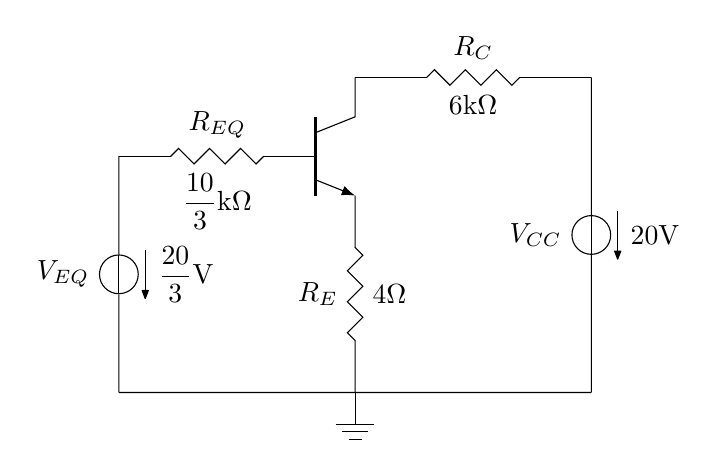
\begin{tikzpicture}[circuit ee IEC,set resistor graphic=var resistor IEC graphic]
\draw (-0.5,0) to [resistor={ohm=\dfrac{10}{3}k,info'=$R_{EQ}$}] (-3,0);
\draw (-3,0) to [voltage source={direction info={volt=\dfrac{20}{3}},info'=$V_{EQ}$}] (-3,-3);
\draw (3,1) to [voltage source={direction info={volt=20},info'=$V_{CC}$}] (3,-3);
\draw (3,1) to [resistor={ohm=6k,info'=$R_C$}] (0,1);
\draw (0,-0.5) to [resistor={ohm=4,info'=$R_E$}] (0,-3);
\draw [very thick] (-0.5,0.5) -- (-0.5,-0.5);
\draw (-3,-3) -- (3,-3) (0,1) -- (0,0.5) -- (-0.5, 0.3);
\draw[-{Latex}] (-0.5,-0.3) -- (0,-0.5);
\draw (0,-3.5) node (gnd) [ground,point down] {};
\draw (gnd) -- (0,-3);
\end{tikzpicture}
\end{center}

Suppose $V_{BE}=0.7V$,
$$I_C=\frac{V_{EQ}-V_{BE}}{\dfrac{R_{EQ}}{\beta_F}+\dfrac{\beta_F+1}{\beta_F}R_E}=\frac{20/3\unit{V}-0.7\unit{V}}{\dfrac{10/3\unit{k\Omega}}{75}+\dfrac{75+1}{75}\cdot4\unit{k\Omega}}\approx1.456\unit{mA}$$
$$I_E=\frac{V_{EQ}-V_{BE}}{\dfrac{R_{EQ}}{\beta_F+1}+R_E}=\frac{20/3\unit{V}-0.7\unit{V}}{\dfrac{10/3\unit{k\Omega}}{75+1}+4\unit{k\Omega}}\approx1.475\unit{mA}$$
$$V_{CE}=V_{CC}-I_CR_C-I_ER_E=20\unit{V}-1.456\unit{mA}\cdot6\unit{k\Omega}-1.475\unit{mA}\cdot4\unit{k\Omega}=5.364\unit{V}$$

So the $Q$ point is $(1.456\unit{mA},\ 5.364\unit{V})$.

\section{}
\begin{center}
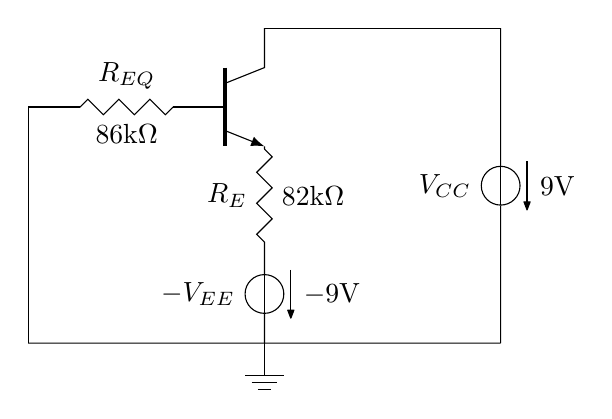
\begin{tikzpicture}[circuit ee IEC,set resistor graphic=var resistor IEC graphic]
\draw (-0.5,0) to [resistor={ohm=86k,info'=$R_{EQ}$}] (-3,0);
\draw (-3,0) -- (-3,-3);
\draw (3,1) to [voltage source={direction info={volt=9},info'=$V_{CC}$}] (3,-3);
\draw (3,1) -- (0,1);
\draw (0,-0.5) to [resistor={near start,ohm=82k,info'=$R_E$},voltage source={near end,direction info={volt=-9},info'=$-V_{EE}$}] (0,-3);
\draw [very thick] (-0.5,0.5) -- (-0.5,-0.5);
\draw (-3,-3) -- (3,-3) (0,1) -- (0,0.5) -- (-0.5, 0.3);
\draw[-{Latex}] (-0.5,-0.3) -- (0,-0.5);
\draw (0,-3.5) node (gnd) [ground,point down] {};
\draw (gnd) -- (0,-3);
\end{tikzpicture}
\end{center}

Suppose $V_{BE}=0.7V$,
$$I_E=\frac{V_{EE}-V_{BE}}{R_E}=\frac{9\unit{V}-0.7\unit{V}}{82\unit{k\Omega}}\approx101\unit{\mu A}$$
$$I_C=\frac{\beta_F}{\beta_F+1}I_E=\frac{100}{100+1}\cdot100\unit{\mu A}$$
$$V_{CE}=V_{CC}-I_CR_C-(-V_{BE})=9\unit{V}+0.7\unit{V}=9.7\unit{V}$$

So the $Q$ point is $(100\unit{\mu A},\ 9.7\unit{V})$.

\section{}
\begin{center}
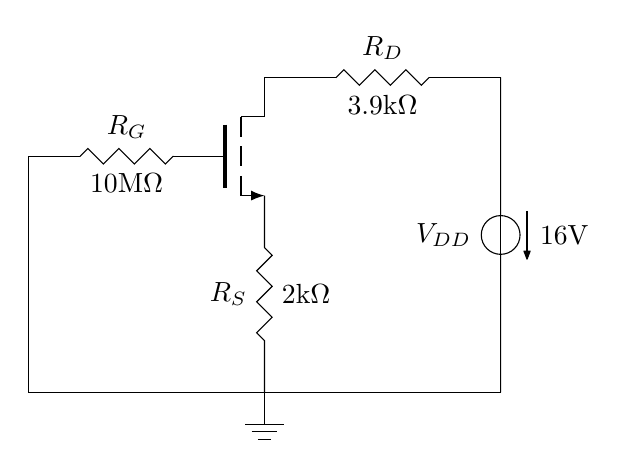
\begin{tikzpicture}[circuit ee IEC,set resistor graphic=var resistor IEC graphic]
\draw (-0.5,0) to [resistor={ohm=10M,info'=$R_G$}] (-3,0);
\draw (-3,0) -- (-3,-3);
\draw (3,1) to [voltage source={direction info={volt=16},info'=$V_{DD}$}] (3,-3);
\draw (3,1) to [resistor={ohm=3.9k,info'=$R_D$}] (0,1);
\draw (0,-0.5) to [resistor={ohm=2k,info'=$R_S$}] (0,-3);
\draw [very thick] (-0.5,0.4) -- (-0.5,-0.4);
\draw (-3,-3) -- (3,-3) (0,1) -- (0,0.5) -- (-0.3, 0.5);
\draw[-{Latex}] (-0.3,-0.5) -- (0,-0.5);
\draw[thick] (-0.3,0.5) -- (-0.3,0.25) (-0.3,0.125) -- (-0.3,-0.125) (-0.3,-0.25) -- (-0.3,-0.5);
\draw (0,-3.5) node (gnd) [ground,point down] {};
\draw (gnd) -- (0,-3);
\end{tikzpicture}
\end{center}

According to the equations,
$$I_D=\frac{K_n}{2}(V_{GS}-V_{TN})^2$$
$$V_{GS}+I_DR_s=0$$

We can get $$V_{GS}+\frac{K_nR_s}{2}(V_{GS}-V_{TN})^2=0$$
$$V_{GS}=V_{TN}=\frac{1}{K_nR_s}\left(\sqrt{1-2K_nR_sV_{TN}}-1\right)$$
\begin{align*}
I_D&=\frac{1}{2K_nR_s^2}\left(\sqrt{1-2K_nR_sV_{TN}}-1\right)^2\\
&=\frac{1}{2\cdot400\unit{\mu A/V^2}\cdot(2\unit{k\Omega})^2}\left(\sqrt{1-2\cdot400\unit{\mu A/V^2}\cdot2\unit{k\Omega}\cdot-5\unit{V}}-1\right)^2\\
&=1.25\unit{mA}
\end{align*}
$$V_{DS}=V_{DD}-I_D(R_D+R_S)=16\unit{V}-1.25\unit{mA}\cdot(3.9\unit{k\Omega}+2\unit{k\Omega})=8.625\unit{V}$$
\begin{align*}
V_{GS}-V_{TN}&=\frac{1}{K_nR_s}\left(\sqrt{1-2K_nR_sV_{TN}}-1\right)\\
&=\frac{1}{2\cdot400\unit{\mu A/V^2}\cdot2\unit{k\Omega}}\left(\sqrt{1-2\cdot400\unit{\mu A/V^2}\cdot2\unit{k\Omega}\cdot-5\unit{V}}-1\right)\\
&=1.25\unit{V}<V_{DS}
\end{align*}

So the $Q$ point is $(1.25\unit{mA},\ 8.625\unit{V})$, and it is in the saturated region.

\section{}
First, we draw the dc equivalent circuit:
\begin{center}
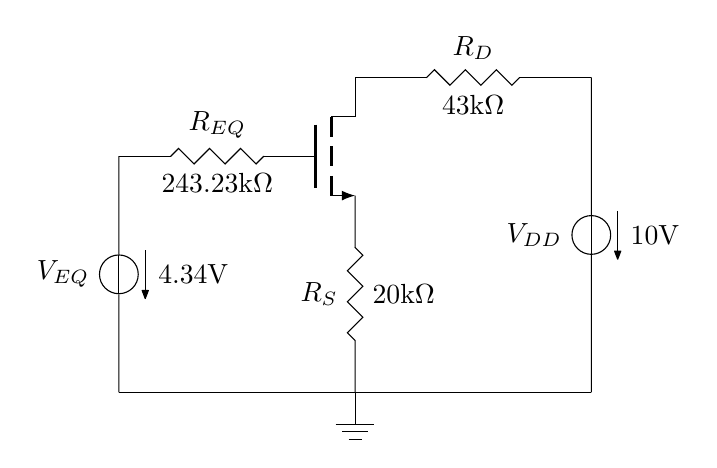
\begin{tikzpicture}[circuit ee IEC,set resistor graphic=var resistor IEC graphic]
\draw (-0.5,0) to [resistor={ohm=243.23k,info'=$R_{EQ}$}] (-3,0);
\draw (-3,0) to [voltage source={direction info={volt=4.34},info'=$V_{EQ}$}] (-3,-3);
\draw (3,1) to [voltage source={direction info={volt=10},info'=$V_{DD}$}] (3,-3);
\draw (3,1) to [resistor={ohm=43k,info'=$R_D$}] (0,1);
\draw (0,-0.5) to [resistor={ohm=20k,info'=$R_S$}] (0,-3);
\draw [very thick] (-0.5,0.4) -- (-0.5,-0.4);
\draw (-3,-3) -- (3,-3) (0,1) -- (0,0.5) -- (-0.3, 0.5);
\draw[-{Latex}] (-0.3,-0.5) -- (0,-0.5);
\draw[thick] (-0.3,0.5) -- (-0.3,0.25) (-0.3,0.125) -- (-0.3,-0.125) (-0.3,-0.25) -- (-0.3,-0.5);
\draw (0,-3.5) node (gnd) [ground,point down] {};
\draw (gnd) -- (0,-3);
\end{tikzpicture}
\end{center}

According to the equations,
$$I_D=\frac{K_n}{2}(V_{GS}-V_{TN})^2$$
$$V_{GS}+I_DR_s=V_{EQ}$$

We can get $$V_{GS}+\frac{K_nR_s}{2}(V_{GS}-V_{TN})^2=V_{EQ}$$
$$V_{GS}=V_{TN}+\frac{1}{K_nR_s}\left(\sqrt{1+2K_nR_s(V_{EQ}-V_{TN})}-1\right)$$
\begin{align*}
I_D&=\frac{1}{2K_nR_s^2}\left(\sqrt{1+2K_nR_s(V_{EQ}-V_{TN})}-1\right)^2\\
&=\frac{1}{2\cdot0.5\unit{mA/V^2}\cdot(20\unit{k\Omega})^2}\left(\sqrt{1+2\cdot0.5\unit{mA/V^2}\cdot20\unit{k\Omega}\cdot(4.34\unit{V}-1\unit{V}})-1\right)^2\\
&\approx131\unit{\mu A}
\end{align*}
$$V_{DS}=V_{DD}-I_D(R_D+R_S)=10\unit{V}-131\unit{\mu A}\cdot(43\unit{k\Omega}+20\unit{k\Omega})\approx1.75\unit{V}$$
\begin{align*}
V_{GS}-V_{TN}&=\frac{1}{K_nR_s}\left(\sqrt{1+2K_nR_s(V_{EQ}-V_{TN})}-1\right)\\
&=\frac{1}{0.5\unit{mA/V^2}\cdot20\unit{k\Omega}}\left(\sqrt{1+2\cdot0.5\unit{mA/V^2}\cdot20\unit{k\Omega}\cdot(4.34\unit{V}-1\unit{V}})-1\right)\\
&\approx0.717\unit{V}<V_{DS}
\end{align*}
So the $Q$ point is $(131\unit{\mu A},\ 1.75\unit{V})$, and it is in the saturated region.

Then we can draw the ac equivalent circuit:
\begin{center}
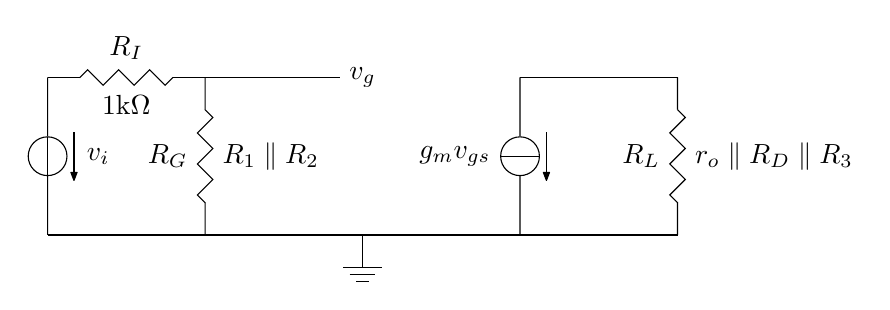
\begin{tikzpicture}[circuit ee IEC,set resistor graphic=var resistor IEC graphic]
\draw (-4,0) to [voltage source={direction info={info=$v_i$}}] (-4,-2);
\draw (-2,0) to [resistor={ohm=1k,info'=$R_I$}] (-4,0);
\draw (-2,0) to [resistor={info=$R_1\parallel R_2$,info'=$R_G$}] (-2,-2);
\draw (0,0) node (vg) {$v_g$};
\draw (-2,0) -- (vg) (-4,-2) -- (4,-2) (4,0) -- (2,0);
\draw (4,0) to [resistor={info=$r_o\parallel R_D\parallel R_3$,info'=$R_L$}] (4,-2);
\draw (2,0) to [current source={direction info={},info'=$g_mv_{gs}$}] (2,-2);
\draw (0,-2.5) node (gnd) [ground,point down] {};
\draw (gnd) -- (0,-2);
\end{tikzpicture}
\end{center}

$$g_m=\frac{2I_D}{V_{GS}-V_{TN}}=\frac{2\cdot131\unit{\mu A}}{0.717\unit{V}}\approx3.65\times10^{-4}\unit{\Omega^{-1}}$$
$$r_o=\frac{\dfrac{1}{\lambda}+V_{DS}}{I_D}=\frac{\dfrac{1}{0.0133\unit{V^{-1}}}+1.75\unit{V}}{131\unit{\mu A}}\approx587\unit{k\Omega}$$
$$R_G=R_1\parallel R_2\approx243.23\unit{k\Omega}$$
$$R_L=r_o\parallel R_D\parallel R_3\approx28.6\unit{k\Omega}$$

The voltage gain is
\begin{align*}
A_v^{CS}&=-g_mR_L\left(\frac{R_G}{R_G+R_I}\right)\\
&=-3.65\times10^{-4}\unit{\Omega^{-1}}\cdot28.6\unit{k\Omega}\cdot\left(\frac{243.23\unit{k\Omega}}{243.23\unit{k\Omega}+1\unit{k\Omega}}\right)\\
&\approx-10.4\unit{dB}
\end{align*}

\section{}
\begin{enumerate}[(a)]
\item $$g_d=\frac{I_S}{V_T}\exp\left(\frac{V_D}{V_T}\right)=\frac{8\unit{fA}}{0.025\unit{V}}\exp\left(\frac{0.6\unit{V}}{0.025\unit{V}}\right)\approx8.48\times10^{-3}\unit{\Omega^{-1}}$$
$$r_d=\frac{1}{g_d}=\frac{1}{8.48\times10^{-3}\unit{\Omega^{-1}}}\approx118\unit{\Omega}$$
\item $$g_d=\frac{I_S}{V_T}\exp\left(\frac{V_D}{V_T}\right)=\frac{8\unit{fA}}{0.025\unit{V}}\exp\left(\frac{0\unit{V}}{0.025\unit{V}}\right)\approx3.2\times10^{-13}\unit{\Omega^{-1}}$$
$$r_d=\frac{1}{g_d}=\frac{1}{3.2\times10^{-13}\unit{\Omega^{-1}}}\approx3.125\times10^{12}\unit{\Omega}$$
\item $$g_d=\frac{I_S}{V_T}\exp\left(\frac{V_D}{V_T}\right)=\frac{1}{r_d}$$
$$V_D=V_T\ln\left(\frac{V_T}{I_Sr_d}\right)=0.025\unit{V}\ln\left(\frac{0.025\unit{V}}{8\unit{fA}\cdot10^{12}\unit{\Omega}}\right)\approx2.85\times10^{-2}\unit{V}$$
\end{enumerate}

\section{}
$$r_\pi=\frac{\beta_oV_T}{I_C}=\frac{100\cdot0.025\unit{V}}{40\unit{\mu A}}=62.5\unit{k\Omega}$$

$$g_m=\frac{I_C}{V_T}=\frac{40\unit{\mu A}}{0.025}=1.6\times10^{-3}\unit{\Omega^{-1}}$$
$$r_o=\frac{1}{g_o}=\frac{V_A+V_{CE}}{I_C}=\frac{75\unit{V}+10\unit{V}}{40\unit{\mu A}}=2125\unit{k\Omega}$$

$$R_L=r_o\parallel R_C\parallel R_3\approx48.85\unit{k\Omega}$$

The input resistance is
$$R_B\parallel r_\pi\approx38.46\unit{k\Omega}$$

The voltage gain is
\begin{align*}
A_v^{CE}&=-g_mR_L\left[\frac{R_B\parallel r_\pi}{R_I+(R_B\parallel r_\pi)}\right]\\
&=-1.6\times10^{-3}\unit{\Omega^{-1}}\cdot48.85\unit{k\Omega}\cdot\left(\frac{38.46\unit{k\Omega}}{750\unit{\Omega}38.46\unit{k\Omega}}\right)\\
&\approx76.7\unit{dB}
\end{align*}

\end{document}

